\documentclass[german,ignorenonframetext
,hideothersubsections %% Im Sidebar nur die aktuellen Subsections anzeigen
]{beamer}

\usepackage[ngerman]{babel} % f�r deutsche Spracheinstellungen
\usepackage{graphics} % um Bilder einbinden zu k�nnen
\usepackage[dvips]{epsfig} % um Bilder zu skalieren
\usepackage[applemac]{inputenc} % inputencoding (MacOS) f�r Umlaute und Akzente
\usepackage{multimedia}

% f�r Code:
\usepackage{listings}
\usepackage{color}

\lstset{ basicstyle=\footnotesize,        % the size of the fonts that are used for the code
  commentstyle=\color{red},    % comment style
%  frame=single,                    % adds a frame around the code
  keepspaces=true,                 % keeps spaces in text, useful for keeping indentation of code (possibly needs columns=flexible)
  keywordstyle=\color{blue},       % keyword style
}

%%%%%%%%%%%%%%%%%%%%%%%%%%%%%%%%%%%%%%%%%%%

%%%%%%% Die folgenden Befehle definieren das Grundlayout, blenden auf der
%%%%%%% Titelseite die HAW-Infos ein und setzen das 
%%%%%%% HAW-Logo in die Ecke
\mode<presentation>{\usetheme{Berkeley}}
\logo{\pgfimage[height=1.5cm]{HAW_wuerfel+}}
\institute[MT -- HAW Hamburg]{HAW Hamburg\\ Dept.\ Informatik}

%%%%%%% der folgende Befehl l�sst die mit "\pause" verdeckten Teile der Folien 
%%%%%%% transparent erscheinen.  
\setbeamercovered{transparent}  

%%%%%%% die folgende Sequenz blendet mit jeder neuen Section einmal das 
%%%%%%% Inhaltsverzeichnis mit dem Titel "�bersicht" ein und markiert den
%%%%%%% jeweils aktuellen Gliederungspunkt
\AtBeginSection[]{
\begin{frame}<beamer>
\frametitle{�bersicht} 
\tableofcontents[currentsection,currentsubsection]
\end{frame}
}

%%%%%%%%%%%%%%%%%%%%%%%%%%%%%%%%%%%%%%%%%%%

%%%%%%% jeder dieser Titelseiten-Befehle kennt eine in eckige Klammern gesetzte 
%%%%%%% Kurzform, die im Rand benutzt wird
\title[Interaktive Schnittstellen]{Interaktive Schnittstellen zu virtuellen Welten}
\subtitle{Projekt im Wintersemester 2013}
\author[]{}
\date{\today}

%%%%%%%%%%%%%%%%%%%%%%%%%%%%%%%%%%%%%%%%%%%

\begin{document}

%%%%%% dieser Befehl erzeugt das Deckblatt. 
%%%%%% Mit der Option plain wird das Layout f�r das Deckblatt abgeschaltet
%\frame[plain]{\titlepage}
\frame{\titlepage}

\begin{frame}
  \frametitle{�bersicht}
  \tableofcontents
\end{frame}

%%%%%%%%%%%%%%%%%%%%%%%%%%%%%%%%%%%%%%%%%%%
%%%%%%%%%%%%%%%%%%%%%%%%%%%%%%%%%%%%%%%%%%%
\section{Hardware} 
%%%%%%%%%%%%%%%%%%%%%%%%%%%%%%%%%%%%%%%%%%%
%%%%%%%%%%%%%%%%%%%%%%%%%%%%%%%%%%%%%%%%%%%


\begin{frame}
\frametitle{Emotiv EEG}

\begin{center}  
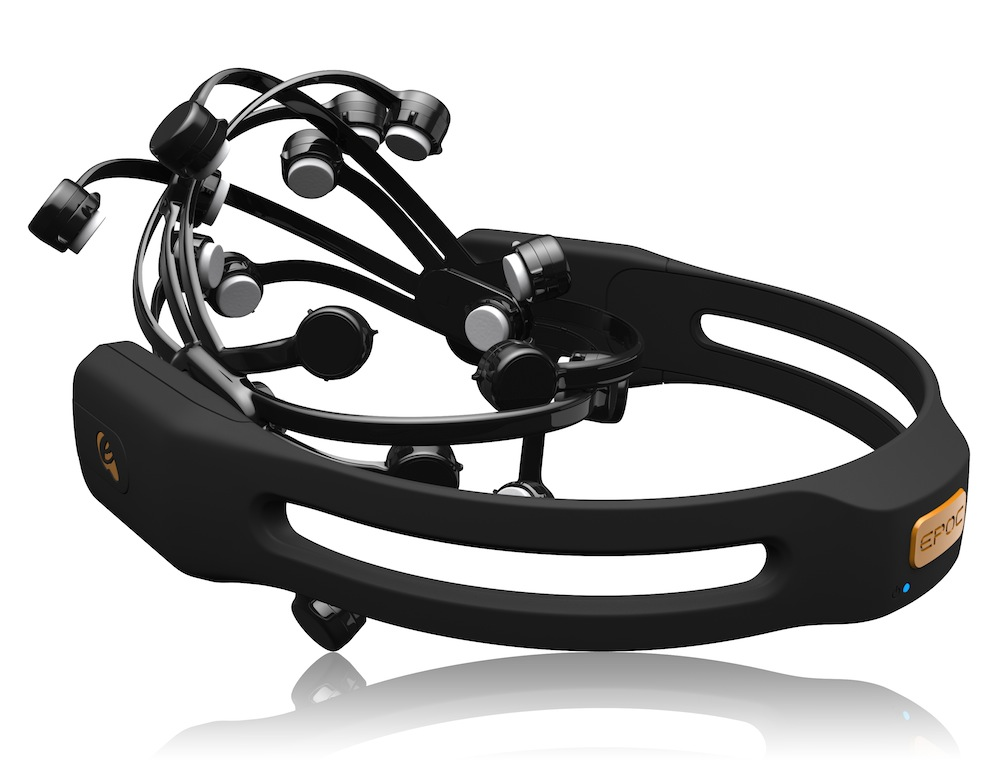
\includegraphics[width=.7\textwidth]{EmotivEEG.jpg}
\end{center}  

\end{frame}


\begin{frame}
  \frametitle{Emotiv-API}
  
  Die Emotiv-API (drei C-Header und entsprechende Binaries) bietet Zugriff auf Daten auf vier veschiedenen Ebenen:
  
\begin{enumerate}
\item rohe Messwerte der 14 Elektroden und des Gyroskops
\item Mimik-Ereignisse (''Expressiv Suite'')
\item ''Emotions-Werte'' (''Affectiv Suite'')
\item trainierte, wiedererkannte ''Gedanken''-Muster (''Cognitiv Suite'')
\end{enumerate} 

Wie die Daten der Ebenen 2-4 berechnet werden, bleibt leider ein Geheimnis der Hersteller-Firma.

\end{frame}

\begin{frame}
\frametitle{Neurosky Mindwave}

\begin{center}  
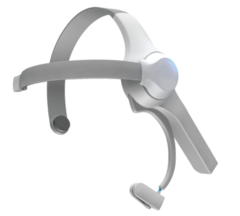
\includegraphics[width=.7\textwidth]{MindWave.png}
\end{center}

\end{frame}


\begin{frame}
\frametitle{Microsoft Kinect}
\begin{center}  
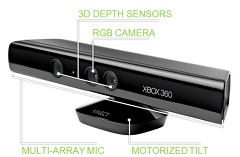
\includegraphics[width=.7\textwidth]{KinectSensor}
\end{center}

\end{frame}

%%%%%%%%%%%%%%%%%%%%%%%%%%%%%%%%%%%%%%%%%%%
%%%%%%%%%%%%%%%%%%%%%%%%%%%%%%%%%%%%%%%%%%%
\section{Signalanalyse} 
%%%%%%%%%%%%%%%%%%%%%%%%%%%%%%%%%%%%%%%%%%%
%%%%%%%%%%%%%%%%%%%%%%%%%%%%%%%%%%%%%%%%%%%

%%%%%%%%%%%%%%%%%%%%%%%%%%%%%%%%%%%%%%%%%%%
%\subsection{bwview}
%%%%%%%%%%%%%%%%%%%%%%%%%%%%%%%%%%%%%%%%%%%

\begin{frame}
\frametitle{Auswertung - erste Versuche}
  
\pgfimage[width=\textwidth]{linplot_linkes_bein.png}
  
\end{frame}

\begin{frame}
\frametitle{bwview}

\begin{center}
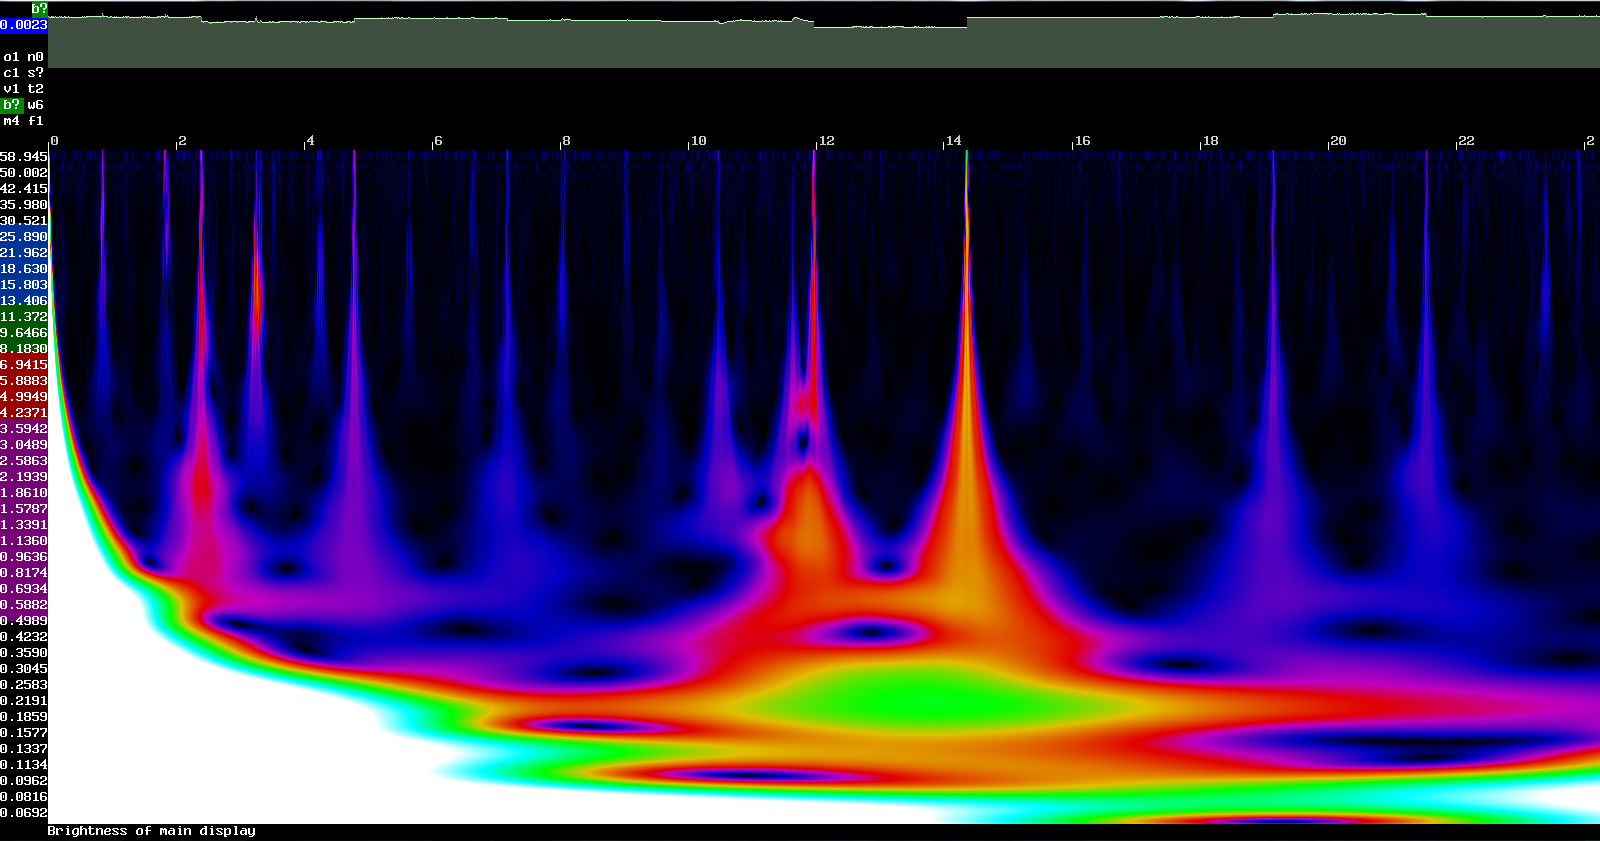
\includegraphics[width=\textwidth]{Video_linkes_Bein.png}
\end{center}

Teil des OpenEEG-Projekts, seit 2007 nicht mehr offiziell weiter entwickelt.
\end{frame}


\begin{frame}[fragile]
\frametitle{bwview - Arbeit am Code}

\begin{block}{Fremder Code ist immer f�r eine �berraschung gut:}
\begin{lstlisting}[language=C, basicstyle=\small]
siz= aa->c.sx * aa->c.tbase + 
        (int)aa->wwid[a] + 2 + 10;
        // +2 for rounding, +10 for luck
\end{lstlisting}
\end{block}

\vspace{\baselineskip}

Unsere Arbeit am Quellcode:

\begin{itemize}
\item Nachvollziehen der Berechnungen
\item Builds und build-Anleitungen f�r aktuelle Betriebssysteme
\item Anpassen an fftw 3.X
\end{itemize}

\end{frame}


%%%%%%%%%%%%%%%%%%%%%%%%%%%%%%%%%%%%%%%%%%%
%\section{Datenanalye Frequenzb�nder und Sensorregionen}
%%%%%%%%%%%%%%%%%%%%%%%%%%%%%%%%%%%%%%%%%%%


%%%%%%%%%%%%%%%%%%%%%%%%%%%%%%%%%%%%%%%%%%%
%%%%%%%%%%%%%%%%%%%%%%%%%%%%%%%%%%%%%%%%%%%
\section{Hardware-Abstraktions-Layer} 
%%%%%%%%%%%%%%%%%%%%%%%%%%%%%%%%%%%%%%%%%%%
%%%%%%%%%%%%%%%%%%%%%%%%%%%%%%%%%%%%%%%%%%%


%%%%%%%%%%%%%%%%%%%%%%%%%%%%%%%%%%%%%%%%%%%
\subsection{Emotiv Epoc API Wrapper} % die sections sind hier nur zum Strukturieren des Vortrags!!
%% der Name der section taucht nur im Inhaltsverzeichnis und im linken Rand auf.
%%%%%%%%%%%%%%%%%%%%%%%%%%%%%%%%%%%%%%%%%%%


\begin{frame}
  \frametitle{Emotiv Epoc API}
  
Die Emotiv Epoc API in ist nativ C geschrieben.
Sie ist dabei jedoch umst�ndlich, und nur m��ig dokumentiert.
\pause
Deswegen: Entwicklung eines Wrappers f�r eine komfortablere Nutzung des EEG Headsets.

\end{frame}

\begin{frame}
  \frametitle{Emotiv Epoc API Wrapper}
  
Der API Wrapper ist in C++ geschrieben.
Bei der Entwicklung wurde auf objektorientierte Prinzipien geachtet.
Es wurde ebenfalls eine allgemeine Schnittstelle definiert, die es erm�glicht mit minimalem Aufwand unterschiedliche EEG Headsets zu nutzen.
Er liefert die Daten f�r den OSC-Server.

\end{frame}

\begin{frame}
  \frametitle{Emotiv Epoc API Wrapper Funktionalit�ten}

  \begin{itemize}
      \item Konzentration
      \item Meditation
      \item Frustration
      \item Aufregung
      \item Einzelwerte der 14 Elektroden
      \item Gyroskop Werte
      \item Timestamp
      \item Counter
   \end{itemize}

\end{frame}


%%%%%%%%%%%%%%%%%%%%%%%%%%%%%%%%%%%%%%%%%%%
\subsection{Verteilte Systeme mit OSC-Kopplung}
%%%%%%%%%%%%%%%%%%%%%%%%%%%%%%%%%%%%%%%%%%%

\begin{frame}
  \frametitle{Aufbau}
  
  \pgfimage[width=\textwidth]{Overview}
  

\end{frame}

\begin{frame}
  \frametitle{OSC}
  
  Wieso Open Sound Control Nachrichten:
  
\begin{enumerate}
\item Plattform- und sprachunabh�ngig
\item die asynchrone Kommunikation verhindert Deadlocks
\item einfacher Aufbau der Nachrichten
\item f�r die meisten Sprachen gibt es Open Source Implementierungen
\end{enumerate} 

\end{frame}

%%%%%%%%%%%%%%%%%%%%%%%%%%%%%%%%%%%%%%%%%%%
%%%%%%%%%%%%%%%%%%%%%%%%%%%%%%%%%%%%%%%%%%%
\section{Anwendungen} 
%%%%%%%%%%%%%%%%%%%%%%%%%%%%%%%%%%%%%%%%%%%
%%%%%%%%%%%%%%%%%%%%%%%%%%%%%%%%%%%%%%%%%%%


%%%%%%%%%%%%%%%%%%%%%%%%%%%%%%%%%%%%%%%%%%%
\subsection{Torcs} % die sections sind hier nur zum Strukturieren des Vortrags!!
%% der Name der section taucht nur im Inhaltsverzeichnis und im linken Rand auf.
%%%%%%%%%%%%%%%%%%%%%%%%%%%%%%%%%%%%%%%%%%%

\begin{frame}
\frametitle{Torcs - The Open Racing Car Simulator}

\begin{center}
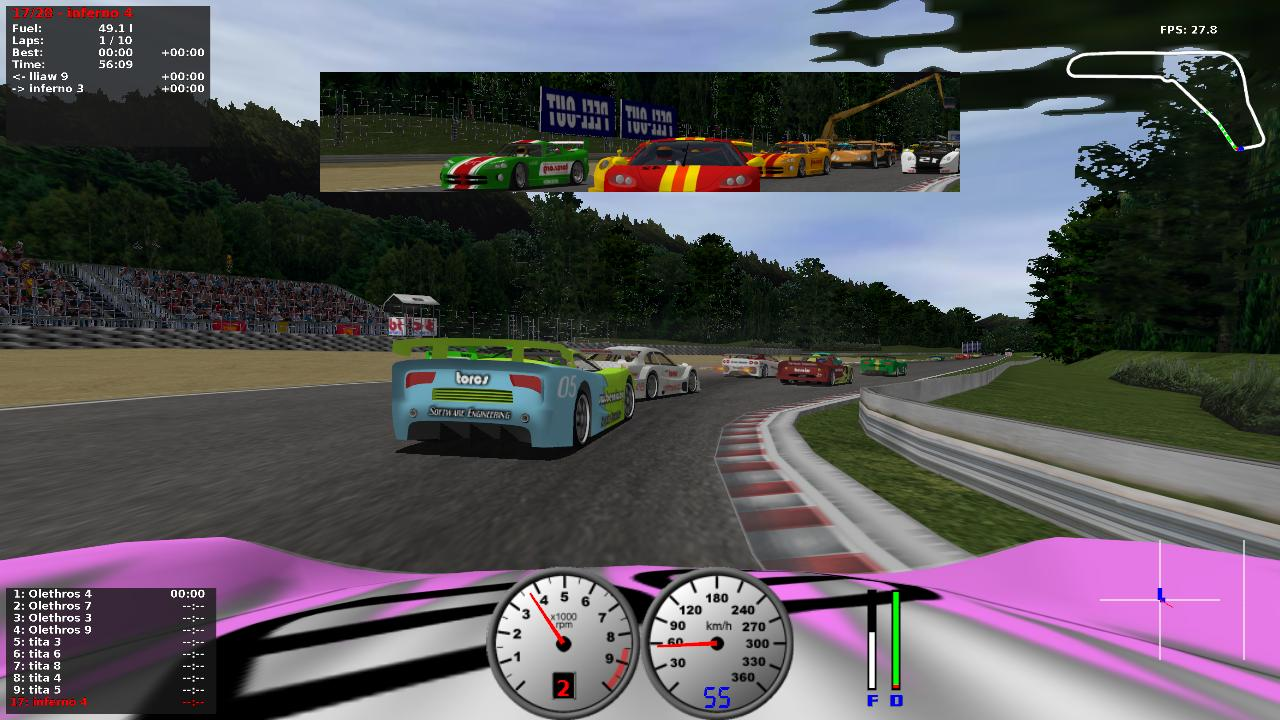
\includegraphics[width=\textwidth]{torcs-screenshot.png}
\end{center}
\end{frame}


\begin{frame}
\frametitle{Torcs - The Open Racing Car Simulator}

%%%%% AUSSCHNEIDEN


\begin{itemize}
\item Open Source Lizenz - GPL
\item 3D Rennspiel
\item Fahrer programmierbar
\item Gaspedalstellung per EEG
\item http://torcs.sourceforge.net/
\end{itemize}
\end{frame}


\begin{frame}
\frametitle{Interaktion}
\begin{center}
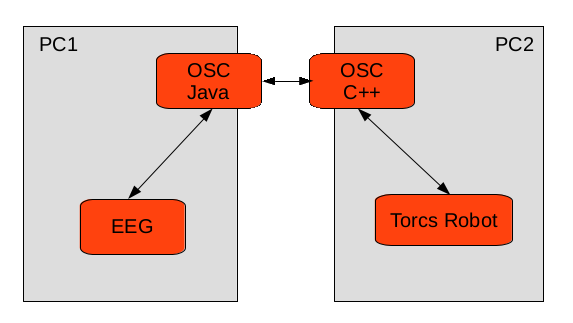
\includegraphics[scale=0.5]{torcs.png}
\end{center}
\end{frame}



%%%%%%%%%%%%%%%%%%%%%%%%%%%%%%%%%%%%%%%%%%%
\subsection{Sonifikation von ''Gedanken''}
%%%%%%%%%%%%%%%%%%%%%%%%%%%%%%%%%%%%%%%%%%%

\begin{frame}

\frametitle{Kooperation mit der HMTM Hannover}       
\begin{center}  
\pgfimage[width=.6\textwidth]{Hochschule_fuer_Musik_und_Theater_Hannover.jpg}
\end{center}  

Vergangene Woche: Besuch von Vincent Michalke, Student f�r Komposition an der HMTM Hannover.

Erste Experimente ''EEG to CSound'' waren erfolgreich - im Folgesemester geht es weiter...


\end{frame}


%%%%%%%%%%%%%%%%%%%%%%%%%%%%%%%%%%%%%%%%%%%
\subsection{Steuerung von Gitarreneffekten}
%%%%%%%%%%%%%%%%%%%%%%%%%%%%%%%%%%%%%%%%%%%

\begin{frame}
\frametitle{Neurosky BCI und Kinect zu OSC}
\begin{center}  
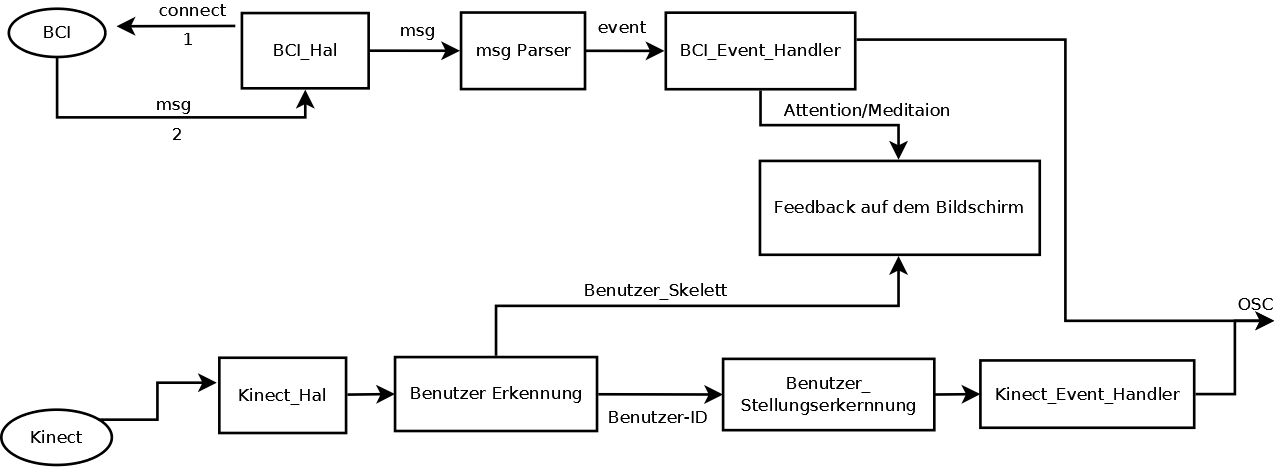
\includegraphics[width=\textwidth]{1-JavaDiagramm.png}
\end{center}

\end{frame}

\begin{frame}
\frametitle{Steuerung der Gitarreneffekte}
\begin{center}  
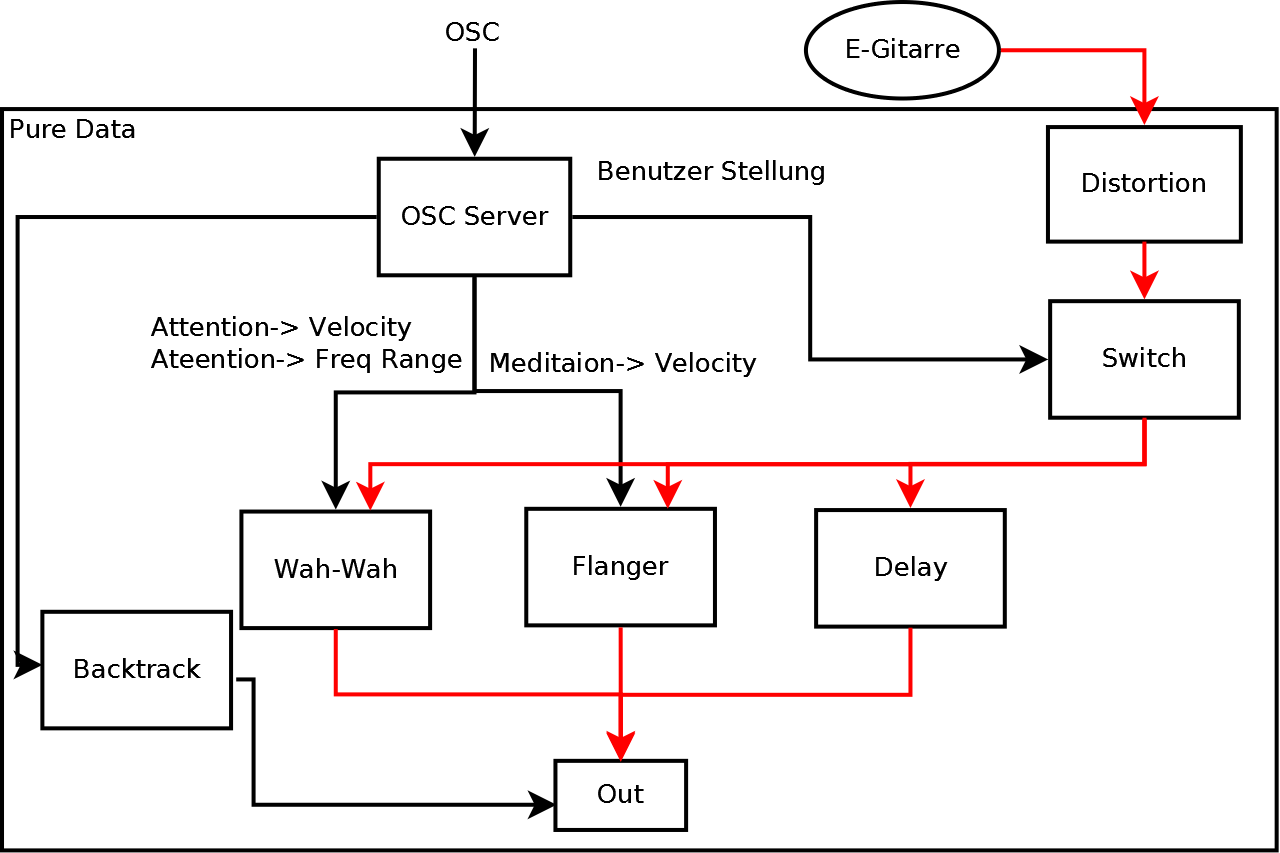
\includegraphics[width=.9\textwidth]{2-Puredata_Diagramm.png}
\end{center}

\end{frame}

\begin{frame}
\frametitle{Gesten f�r Kinect}
\begin{center}  
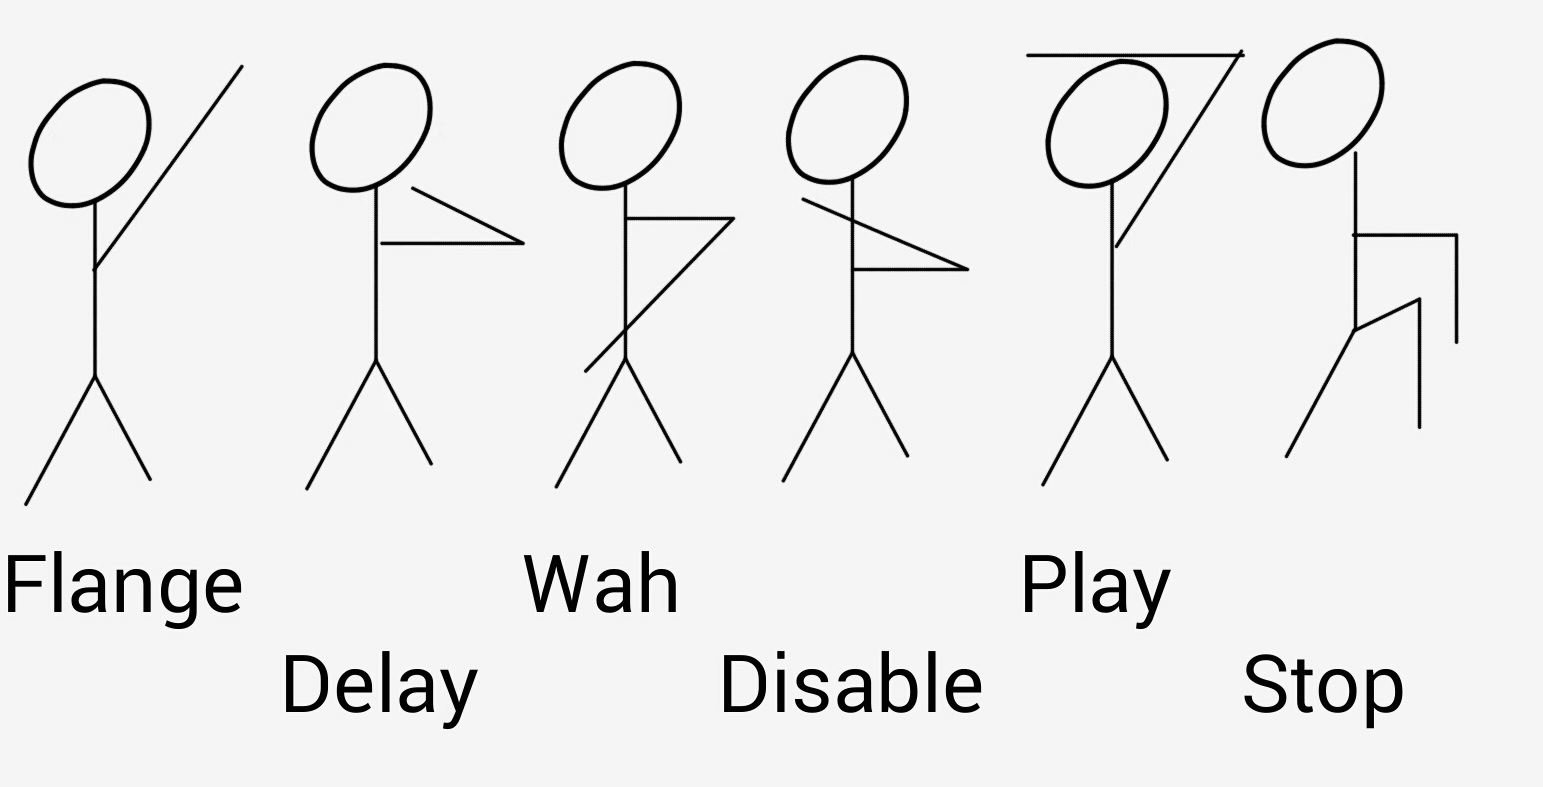
\includegraphics[width=\textwidth]{3-Stellungen.jpg}
\end{center}

\end{frame}


\end{document} %%%%% END DOCUMENT %%%%%%


%%%%%%%%%%%%%%%%%%%%%%%%%%%%%%%%%%%%%%%%%%%
%%  besondere Gestaltungselemente f�r Vortragsfolien
%%%%%%%%%%%%%%%%%%%%%%%%%%%%%%%%%%%%%%%%%%%

% Folie
\begin{frame}
\frametitle{Folientitel}
        Text, Bilder, Bl�cke
\end{frame}

% neutraler Kasten
\begin{block}{Blocktitel}
        Blocktext
\end{block}

% gr�ner Kasten
\begin{exampleblock}{Beispielblocktitel}
        Beispielblocktext
\end{exampleblock}

% roter Kasten
\begin{alertblock}{Warnungsblocktitel}
        Warnungsblocktext
\end{alertblock}

% mehrspaltige Folie mit variablen Spaltenbreiten
\begin{columns}
\column{.55\textwidth}
        Text oder Bild
\column{.45\textwidth}
        Text oder Bild
\end{columns}

% sukzessiver Folienaufbau 
\pause

% mehr Befehle f�r sukzessiven Folienaufbau, 
% der geklammerte Teil erscheint jeweils ab der dritten Teil-Folie
\uncover<3->{}
\only<3->{}
\invisible<1-2>{}

% rote Markierung des geklammerten Teils bei der vierten Teil-Folie
\alert<4>{}

%%%%%%%%%%%%%%%%%%%%%%%%%%%%%%%%%%%%%%%%%%%